\documentclass[a4paper,12pt]{article}
\usepackage[swedish]{babel}
\usepackage[utf8]{inputenc}
\usepackage{amsmath, amsthm, amssymb}
\usepackage{graphicx}
\usepackage{enumitem}
\usepackage[a4paper,includeheadfoot,margin=2.54cm]{geometry}
\usepackage{fancyhdr}
\pagestyle{fancy}
\fancyhead[R]{Zacharias Brohn - 9907174297}
\renewcommand{\headrulewidth}{0pt}
\setlength{\headheight}{14.5pt}
%
\begin{document}
%
\section*{Dugga 8 - Fråga 0}
Bestäm samtliga lösningar till
\begin{align*}
    33x + 3 \equiv 11 \mod{91}.
\end{align*}
\subsection*{Lösning}
Vi börjar med att subtrahera 3 från båda sidor av ekvationen
\begin{align}
    33x + 3 &\equiv 11 \mod{91} \\
    33x &\equiv 8 \mod{91}. \label{eq1}
\end{align}
Nu kan vi använda den utökade Euklidiska algoritmen för att hitta positiva $x$,
och algoritmen ser ut som sådan
\begin{align}
    \text{GCD}(a,~b) = ax + by
\end{align}
där vi itererar genom följande
\begin{align}
    q_i = \left\lfloor \frac{a_i}{b_i} \right\rfloor, \quad r_i = a_i \mod{b_i}
\end{align}
där $q$ är kvoten av $a$ genom $b$ och $r$ är resten. Vi initierar koefficienterna
\begin{align}
    x_0 = 1, \quad y_0 = 0, \quad x_1 = 0, \quad y_1 = 1
\end{align}
och för varje $i$ uppdaterar vi koefficienterna enligt
\begin{align}
    x_{i+1} = x_{i-1} - q_ix_i, \quad y_{i+1} = y_{i-1} - q_iy_i.
\end{align}
Alltså, vi börjar med $q_1$ och fortsätter tills vi får en rest $r_i = 0$.
Första iterationen
\begin{gather}
    q_1 = \left\lfloor \frac{91}{33} \right\rfloor = 2,~r_1 = 91 \mod 33 = 25 \\
    a_1 = 33,~b_1 = 25 \\
    x_2 = x_0 - q_1x_1 = 1 - 2 \cdot 0 = 1,~y_2 = y_0 - q_1y_1 = 0 - 2 \cdot 1 = -2 \\
\end{gather}
andra iterationen
\begin{gather}
    q_2 = \left\lfloor \frac{33}{25} \right\rfloor = 1,~r_2 = 33 \mod 25 = 8 \\
    a_2 = 25,~b_2 = 8 \\
    x_3 = 0 - 1 \cdot 1 = -1,~y_3 = 1 - 1 \cdot (-2) = 3
\end{gather}
tredje iterationen
\begin{gather}
    q_3 = \left\lfloor \frac{25}{8} \right\rfloor = 3,~r_3 = 25 \mod 8 = 1 \\
    a_3 = 8,~b_3 = 1 \\
    x_4 = 1 - 3 \cdot (-1) = 4,~y_4 = -2 - 3 \cdot 3 = -11
\end{gather}
fjärde iterationen
\begin{gather}
    q_4 = \left\lfloor \frac{8}{1} \right\rfloor = 8,~r_4 = 8 \mod 1 = 0.
\end{gather}
Eftersom $r_4 = 0$ så har vi funnit koefficienterna $x_4 = 4$ och
$y_4 = -11$. Vi letar efter den positiva
lösningen så vi adderar med $91$
\begin{gather}
    -11 + 91 = 80
\end{gather}
om vi nu multiplicerar höger- och vänsterled i ekv.\ref{eq1} med $80$ för att hitta $x$
\begin{align}
    33x \cdot 80 &= 8 \cdot 80 \mod 91 \\
    2640x &= 640 \mod 91
\end{align}
och eftersom
\begin{align*}
    2640 \mod 91 = 1
\end{align*}
kan vi utveckla till
\begin{align*}
    x &= 640 \mod 91 \\
    x &= 3 \mod 91.
\end{align*}
%
\subsection*{Svar}
Den positiva lösningen är $x = 3$. \\
%
\newpage
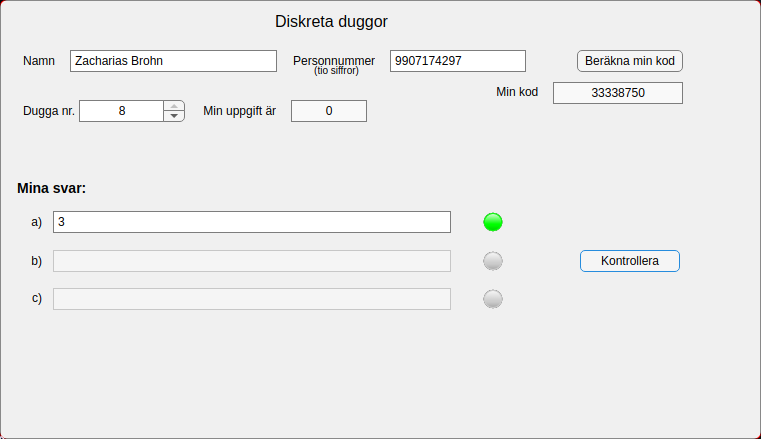
\includegraphics[width=\textwidth]{Nn7932X.png}
\end{document}